\documentclass[letterpaper,12pt]{article}
\usepackage{tabularx} % extra features for tabular environment
\usepackage{graphicx} % takes care of graphic including machinery
\usepackage[margin=1in,letterpaper]{geometry} % decreases margins
\usepackage{cite} % takes care of citations
\usepackage[final]{hyperref} % adds hyper links inside the generated pdf file
\hypersetup{
	colorlinks=true,       % false: boxed links; true: colored links
	linkcolor=blue,        % color of internal links
	citecolor=blue,        % color of links to bibliography
	filecolor=magenta,     % color of file links
	urlcolor=blue         
}
\usepackage{physics}
\usepackage{blindtext}
\usepackage{amssymb}
\usepackage{amsthm}
\usepackage{amsmath}
\usepackage{mathtools}
\usepackage{bm}
% package for Feynman diagrams
\usepackage{tikz-feynman, contour}
\usepackage{tikz}
%++++++++++++++++++++++++++++++++++++++++

\newcommand{\crossvertex}[1]{
    \draw[ultra thick] (#1) ++(-0.1,-0.1) -- ++(0.2,0.2);
    \draw[ultra thick] (#1) ++(-0.1,0.1) -- ++(0.2,-0.2);
}

\begin{document}
\setlength\parindent{0pt}
\setlength\belowdisplayskip{12pt}
\setlength\belowdisplayshortskip{12pt}

\title{An Introduction to Information Field Theory}
\author{Joe Gillett, Uli Raudales \\ Department of Physics, Whitman College}
\date{July 2024}

\maketitle
\section{Information Field Theory Basics}
\subsection{Introduction}
Throughout physics, astronomy and engineering, countless problems exist which can be expressed in the form of continuous random fields. Such fields model systems which exhibit spatial and temporal variation. Many of these fields follow a given distribution, namely the Gaussian distribution, with properties of the field being determined by inferring the parameters of the first two moments (mean and variance) of the distribution. Some systems, however, fail to follow a known distribution, and are thus more difficult to solve for. 
\hfill \break

Irrespective of the form of the model, inference over a continuous field is typically required, as data is collected at discrete points on the domain. Bayes theorem can be used for this purpose, given by the following equation:

\begin{equation}
    P(A|B) = \frac{P(B|A)P(A)}{P(B)}    
\end{equation}

While this approach works well for parameterized random fields, it becomes infeasible in the case of a non-parameterized, non-Gaussian distribution. Calculation of the evidence $P(B)$ requires integrating the joint probability $P(B|A)P(A)$ over all possible values of the field, which is defined on a continuous underlying space. Since this is impractical computationally, another approach must be found. Conventionally, Markov Chain Monte Carlo (MCMC) or related numerical techniques are used in order to circumvent this issue and infer the moments. While this procedure certainly works, it becomes increasingly computationally intensive as the number of parameters increases. 
\hfill \break

Presented is an alternative method of calculating the moments using Bayes-derived techniques from Information Field Theory. Diagrammatic expansion, one such technique, characterizes the posterior moments as an infinite sum of diagrams, each of which corresponds to an equation dependant on the diagram's structure. While this technique does require discretization of the field, the result approaches the continuous limit given sufficient resolution. Additionally, direct calculation of the evidence using a similar technique involving closed diagram expansion is also explored, alongside a potential set of basis functions for more efficient calculations. It should be noted that these techniques require the posterior random field to be perturbatively non-Gaussian, or in other words deviate only slightly from the Gaussian distribution. It is possible that these techniques may work on other named distributions, but to date this has not been tested. 
\subsection{The Diagrammatic Expansion Technique}

The motivation behind many of information field theortic techniques stem from the mathematical similarity between Bayesian inference and that of probabilistic treatment of physical fields. Similar to the Bayes Formula (Eq(1)) the probability of a physical field being in a certain
configuration has been expressed in the following form, often called the Gibbs measure,
\begin{equation}
    P(\bm{x}) = \frac{e^{H(\bm{x})}}{Z(s)} \equiv \frac{P(B | A)P(A)}{P(B)}
\end{equation}

where $H(\bm{x})$ is the Hamiltonian of the field, and $Z$ is the partition function. 
The Hamiltonian is a functional of the field, and is often expressed as a sum of terms, each of which is a function of the field at a certain point in space. 
\begin{equation}
    H(\bm{x}) = \sum_{i} H_{i}(\bm{x}) \equiv -\log P(B|A)P(A)
\end{equation}
The partition function is the normalization constant, and is given by the integral of the exponential of the Hamiltonian over all possible field configurations. 

\begin{equation}
    Z (\bm{s})= \int_{-\infty}^{\infty} d\bm{x} \, e^{-H(\bm{x}) + \bm{s}^{T}\bm{x}}
\end{equation}

where $\bm{s}$ is a book-keeping vector that keeps track of the moments of the field.
The term $\bm{s}^{T}\bm{x}$ acts as a pertubation in the Hamiltonian.
Given the similarity between the partition function and the moment-generating function, it is possible to calculate the moments of the field by taking derivatives of the partition function with respect to the book-keeping vector.
\begin{equation}
    \expval{ x_{1} \dots x_{n} } = \mu_{n} = \frac{1}{Z(\bm{s})}\pdv{^{n}Z(\bm{s})}{s_{1} \dots \partial s_{n}}\Bigg|_{\bm{s}=0} = \pdv{^{n}\log Z(\bm{s})}{s_{1} \dots \partial s_{n}}\Bigg|_{\bm{s}=0}
\end{equation}

For most practical cases, the partition function $Z(s)$ cannot be computed in a closed-form analytical expression, making it highly difficult to extract the moments of the distribution using Eq(4).
However, the diagrammatic expansion technique provides us a method to extract information about the moments from the partition function up to a certain order of accuracy. 
To do so, we begin by expanding the Hamiltonian in a Taylor series expansion,

\begin{equation}
    H(\bm{x}) = H_{0} - \bm{j}^{T}\bm{x} + \frac{1}{2}\bm{x}^{T}\bm{D}^{-1}\bm{x} + \sum_{n=3}^{\infty} \frac{1}{n!} \bm{\Lambda^{(n)}}_{x_{1} \dots x_{n}}\bm{x}^{n}
\end{equation}

where 
\begin{eqnarray}
    \bm{j}(x_{1}) &= -\pdv{H}{x_{1}} \Big|_{\bm{x}=0} \\
    \bm{D}^{-1}(x_{1}, x_{2}) &= \pdv{^{2}H}{x_{1} \partial x_{2}} \Big|_{\bm{x}=0} \\
    \bm{\Lambda^{(n)}}_{x_{1} \dots x_{n}} &= \pdv{^{n}H}{x_{1} \cdots \partial x_{n}} \Big|_{\bm{x}=0}
\end{eqnarray}
In this expression, $\bm{j}(x_{1})$ represents the source of information where the field's influence is most pronounced. The term $\bm{D}^{-1}(x_{1}, x_{2})$ acts as the propagator, functioning similarly to a covariance, facilitating the influence of the random field at location $x_{1}$ on the field at location $x_{2}$. 
The higher-order interactions are encapsulated by the tensors $\bm{\Lambda^{(n)}}_{x_{1} \cdots x_{n}}$, referred to as the nth-order interaction coefficients. These coefficients quantify the contribution's magnitude of the nth power of the random field within the Hamiltonian framework. 
Repeated indices are integrated over (Einstein summation convention), and the nth-order interaction coefficients are symmetric under permutation of their indices.
\begin{equation}
    \Lambda^{(n)}_{x_{1} \dots x_{n}} x_{1} \dots x_{n} = -\int_{-\infty}^{\infty} dx_{1} \cdots dx_{n} \, \Lambda^{(n)}_{x_{1} \dots x_{n}} x_{1} \dots x_{n} 
\end{equation}
In a discrete setting, $\bm{j}$ is a vector, $\bm{D}^{-1}$ is a matrix, and $\bm{\Lambda^{(n)}}$ is a tensor. For discrete cases we summed over repeated indices as per the Einstein summation convention. For example,

\[
M_{ij}A_{i}B_{j} = \sum_{i,j}M_{ij}A_{i}B_{j}
\]
To solve this numerically, we will be dealing with the discrete cases.

\vspace*{0.5cm}
We break the Hamiltonian into two parts, 
$$H_{G}(\bm{x}) = H_{0} - \bm{j}^{T}\bm{x} + \frac{1}{2}\bm{x}^{T}\bm{D}^{-1}\bm{x}$$
which is the Gaussian part of the Hamiltonian, and 
$$H_{I}(\bm{x}) = \sum_{n=3}^{\infty} \frac{1}{n!} \bm{\Lambda^{(n)}}_{x_{1} \dots x_{n}} \bm{x}^{n}$$
which is the interaction part of the Hamiltonian.
Following this, we can write the partition function as a sum of the Gaussian and interaction partition functions,
\begin{align}
    Z(\bm{s}) &= \int_{-\infty}^{\infty} d\bm{x} \, e^{-H(\bm{x}) + \bm{s}^{T}\bm{x}} \\
    &= \int_{-\infty}^{\infty} d\bm{x} \, e^{-(H_{0} - \bm{j}^{T}\bm{x} + \frac{1}{2}\bm{x}^{T}\bm{D}^{-1}\bm{x} + \sum_{n=3}^{\infty} \frac{1}{n!} \bm{\Lambda^{(n)}}_{x_{1} \dots x_{n}} \bm{x}^{n}) + \bm{s}^{T}\bm{x}} 
\end{align}
we note that since $\bm{s}$ enters with a linear power of $\bm{x}$ in the Gaussian exponential, and hence derivatives with respect to $\bm{s}$ will bring down powers of $\bm{x}$. 

\begin{align}
    Z(\bm{s}) &= \exp[-\sum_{n=3}^{\infty} \frac{1}{n!} \bm{\Lambda^{(n)}}_{x_{1} \dots x_{n}} \pdv{^{n}}{x_{1} \cdots \partial x_{n}}] \int_{-\infty}^{\infty} d\bm{x} \, e^{-H_{G}(\bm{x}) + \bm{s}^{T}\bm{x}} \\
    &= \exp[-H_{I}\left(\pdv{^{n}}{x_{1} \cdots \partial x_{n}}\right)] Z_{G}(\bm{s})
\end{align}
\subsection{Feynman Diagrams}

Borrowing from Quantum Field Theory, we can represent the partition function as a sum of diagrams, each of which corresponds to a term in the expansion of the partition function.

\vspace*{0.5cm}
Given that the Gaussian partition function takes the form 
\begin{equation}
    \int_{-\infty}^{\infty} dx \, e^{-ax^{2} + bx + c} = \sqrt{\frac{\pi}{a}} e^{\frac{b^{2}}{4a} + c}
\end{equation}
it can show that the Gaussian partition function has the following exact form,
\begin{equation}
    Z_{G}(\bm{s}) = \sqrt{\abs{2\pi \bm{D}}} \exp[\frac{1}{2}(\bm{s} + \bm{j})^{T}\bm{D}(\bm{s} + \bm{j}) - H_{0}]
\end{equation}


To get the diagrammatic expansion of the partition function, we take the natural logarithm of the partition function 
\begin{equation}
    \log Z_{G}(\bm{s}) = \frac{1}{2}(\bm{s}^{T}\bm{D}\bm{s} + \bm{j}^{T}\bm{D}\bm{s} + \bm{s}^{T}\bm{D}\bm{j} + \bm{j}^{T}\bm{D}\bm{j}) - H_{0} + \log \sqrt{\abs{2\pi \bm{D}}}
\end{equation}

\vspace*{0.5cm}
We represent each information source $\bm{j}$ as 

\begin{tikzpicture}
    \begin{feynman}
        \vertex (a) at (0,0);
        % Use the new command to draw a cross at vertex a
        \crossvertex{a}
    \end{feynman}
\end{tikzpicture}
and each external source $\bm{s}$ as
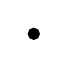
\begin{tikzpicture}
    \begin{feynman}
        \vertex (a) at (0,0);
        % draw a filled circle around the vertex a
        \node[circle,draw,fill=black,inner sep=0.5mm] at (a) {};
    \end{feynman}
\end{tikzpicture}
and each propagator $\bm{D}$ as
\begin{tikzpicture}
    \begin{feynman}
        \vertex (a) at (0,0);
        \vertex (b) at (1,0);
        \diagram* {
            (a) -- (b)
        };
    \end{feynman}
\end{tikzpicture}
and each interaction $\bm{\Lambda^{(n)}}$ as a vertex with $n$ lines coming out of it.

Thus, the diagrammatic expansion of the Gaussian partition function is given by 
\begin{equation}
    \log Z_{G}(\bm{s}) = \frac{1}{2}(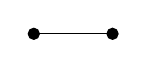
\begin{tikzpicture}
        \begin{feynman}
            \vertex (a) at (0,0);
            \vertex (b) at (1,0);
            \diagram* {
                (a) -- (b)
            };
            \node[circle,draw,fill=black,inner sep=0.5mm] at (a) {};
            \node[circle,draw,fill=black,inner sep=0.5mm] at (b) {};
        \end{feynman}
    \end{tikzpicture} + 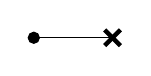
\begin{tikzpicture}
        \begin{feynman}
            \vertex (a) at (0,0);
            \node[circle,draw,fill=black,inner sep=0.5mm] at (a) {};
            \vertex (b) at (1,0);
            \crossvertex{b}
            \diagram* {
                (a) -- (b)
            };
        \end{feynman}
    \end{tikzpicture} + 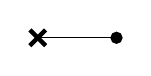
\begin{tikzpicture}
        \begin{feynman}
            \vertex (a) at (0,0);
            \vertex (b) at (1,0);
            \node[circle,draw,fill=black,inner sep=0.5mm] at (b) {};
            \crossvertex{a}
            \diagram* {
                (a) -- (b)
            };
        \end{feynman}
    \end{tikzpicture} + 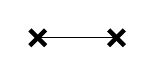
\begin{tikzpicture}
        \begin{feynman}
            \vertex (a) at (0,0);
            \vertex (b) at (1,0);
            \crossvertex{a}
            \crossvertex{b}
            \diagram* {
                (a) -- (b)
            };
        \end{feynman}
    \end{tikzpicture}) - H_{0} + \log \sqrt{\abs{2\pi \bm{D}}}
\end{equation}

Getting the moments of the field is now a matter of taking derivatives of the partition function with respect to the book-keeping vector $\bm{s}$ and evaluating at $\bm{s}=0$.
This is equivalent to counting the number of external sources in the diagram with respect to which we are taking the derivative and removing them from the diagram and evaluating the diagram at $\bm{s}=0$.
So the first moment of the field is given by
\begin{equation}
    \mu_{1} = \pdv{\log Z_{G}(\bm{s})}{s_{1}}\Big|_{\bm{s}=0} = \bm{D}\bm{j} = 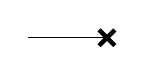
\begin{tikzpicture}
        \begin{feynman}
            \vertex (a) at (0,0);
            \vertex (b) at (1,0);
            % \node[circle,draw,fill=black,inner sep=0.5mm] at (a) {};
            \crossvertex{b}
            \diagram* {
                (a) -- (b)
            };
        \end{feynman}
    \end{tikzpicture} = \int_{-\infty}^{\infty} dx_{1} \, D(x, x_{1})j(x_{1})
\end{equation}

Finding the diagrammatic expansion of the Interactive partition function just requires one to find which which nth-order terms contribute (i.e $\bm{\Lambda^{(n)}} \neq 0$) and then sum over all possible diagrams that can be formed from these terms.
Each diagram is multiplied by a symmetry factor, which is the number of ways the diagram can be drawn without changing its appearance.
\section{IFT in Practice}
\subsection{1D case}
This section explores the implementation of the diagrammatic expansion technique in the 1-dimensional case. While the problem itself is trivial, it should allow for an easy-to-follow, verifiable example of the technique, which can subsequently be used in higher-dimensional cases. Rather than beginning with a data set, instead consider the following non-Gaussian probability density function:

\begin{equation}
    Q(x) = \exp[\frac{-(x - x_{0})^{2}}{2\sigma^2}-bx^4]
\end{equation}

This probability distribution is largely Gaussian, with the $-bx^4$ term slightly perturbing the system. The normalized form of the probability density function is given by:

\begin{equation}
    P(x) = \frac{Q(x)}{Z} = \frac{e^{-H(x)}}{\int_{-\infty}^{\infty} e^{-H(x)} dx}
\end{equation}
Thus we have that the Hamiltonian is given by:

\begin{equation}
    H(x) = \frac{(x - x_{0})^{2}}{2\sigma^2} + bx^4
\end{equation}
Where the second term is the interaction term due to the pertubation.

Taylor expanding the Hamiltonian about $x = 0$ gives:

\begin{equation}
    H(x) = \frac{x^{2}}{2\sigma^2} - \frac{x_{0} x}{\sigma^2} + \frac{x_{0}^{2}}{2\sigma^2} + b x^{4} 
\end{equation}
where 
\begin{align*}
    H_{0} = \frac{x_{0}^{2}}{2\sigma^{2}} \\
    j = -\pdv{H}{x} \Big|_{x=0} &= \frac{x_{0}}{\sigma^2} \\
    D^{-1} = \pdv{^{2}H}{x^{2}} \Big|_{x=0} &= \frac{1}{\sigma^2} \\
    \Lambda^{(4)} = \pdv{^{4}H}{x^{4}} \Big|_{x=0} &= 4!b \\
    \Lambda^{(n \geq 5)} = \Lambda^{(3)} &= 0
\end{align*}
The derivative of $H(x)$ is,
\begin{equation}
    \frac{dH(x)}{dx} \: = \: \frac{x}{\sigma^{2}} - \frac{x_{0}}{\sigma^{2}} + 4bx^{3} \: .
\end{equation}
Since the interaction Hamiltonian is the sum over all possible diagrams formed by the contributing nth-order terms, we have contributions from diagrams $(\Lambda^{(4)})^{n}$ for $n \geq 1$.
So we will have contributions from nth-order terms that are powers of $4n$.

So the log of the partition function would be the sum of all diagrams that can be formed from the nth-order terms and the Gaussian partition function.

\vspace*{0.5cm}
To better understand, let us calculate the first moment of the field, $\mu_{1}$.

\begin{align}
    \mu_{1} &= 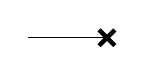
\begin{tikzpicture}[baseline=(current bounding box.center)]
        \begin{feynman}
            \vertex (a) at (0,0);
            \vertex (b) at (1,0);
            \crossvertex{b}
            \diagram* {
                (a) -- (b)
            };
        \end{feynman}
    \end{tikzpicture} + \frac{1}{3!}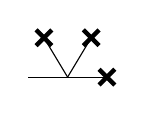
\begin{tikzpicture}[baseline=(current bounding box.center)]
        \begin{feynman}
            \vertex (a) at (0,0);
            \vertex (b) at (0.2,0.5);
            \vertex (e) at (0.5,0);
            \vertex (c) at (0.8,0.5);
            \vertex (d) at (1,0);
            \crossvertex{b}
            \crossvertex{c}
            \crossvertex{d}
            \diagram* {
                (b) -- (e) -- (c) 
            };
            \diagram* {
                (a) -- (e) -- (d)
            };
        \end{feynman}
    \end{tikzpicture} + \frac{1}{4!}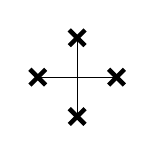
\begin{tikzpicture}[baseline=(current bounding box.center)]
        \begin{feynman}
            \vertex (a) at (0,0);
            \vertex (b) at (0.5,0.5);
            \vertex (e) at (0.5,0);
            \vertex (c) at (0.5,-0.5);
            \vertex (d) at (1,0);
            \crossvertex{a}
            \crossvertex{b}
            \crossvertex{c}
            \crossvertex{d}
            \diagram* {
                (b) -- (e) -- (c) 
            };
            \diagram* {
                (a) -- (e) -- (d)
            };
        \end{feynman}
    \end{tikzpicture} + \frac{1}{2}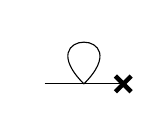
\begin{tikzpicture}[baseline=(current bounding box.center)]
        \begin{feynman}
            \vertex (a) at (0,0);
            \vertex (e) at (0.5,0);
            \vertex (d) at (1,0);
            \crossvertex{d}
            \diagram* {
                (a) -- (e) -- (d),
                (e) -- [out=45,in=135,loop,min distance=1cm] e % Loop at vertex e
            };
        \end{feynman}
    \end{tikzpicture} + \frac{1}{8}\begin{tikzpicture}[baseline=(current bounding box.center)]
        \begin{feynman}
            \vertex (e) at (0,0);
            \diagram* {
                (e) -- [out=135,in=225,loop,min distance=1cm] e, % Left loop
                (e) -- [out=45,in=-45,loop,min distance=1cm] e, % Right loop
            };
        \end{feynman}
    \end{tikzpicture} + \frac{1}{8!}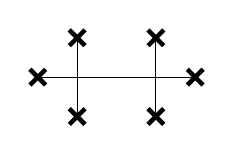
\begin{tikzpicture}[baseline=(current bounding box.center)]
        \begin{feynman}
            \vertex (a) at (0,0);
            \vertex (b) at (0.5,0.5);
            \vertex (e) at (0.5,0);
            \vertex (c) at (0.5,-0.5);
            \vertex (d) at (1,0);
            \vertex (f) at (1.5,0);
            \vertex (g) at (2,0);
            \vertex (h) at (1.5,0.5);
            \vertex (i) at (1.5,-0.5);
            \crossvertex{a}
            \crossvertex{b}
            \crossvertex{c}
            \crossvertex{g}
            \crossvertex{h}
            \crossvertex{i}
            \diagram* {
                (a) -- (e) -- (d) -- (f) -- (g),
                (b) -- (e) -- (c),
                (h) -- (f) -- (i)
            };
        \end{feynman}
    \end{tikzpicture} + \cdots \\
    &= Dj + \frac{1}{3!}D^{3}\Lambda^{(4)}j^{3} + \frac{1}{4!}D^{4}\Lambda^{(4)}j^{4} + \frac{1}{2}D^{2}\Lambda^{(4)}j + \frac{1}{8}D^{2}\Lambda^{(4)} + \frac{1}{8!}D^{6}(\Lambda^{(4)})^{2}j^{7} + \cdots
\end{align}

Since this is a 1-dimensional case, the propagator $D$ is just a scalar, and the interaction term $\Lambda^{(4)}$ is also a scalar.

\subsection{Linear Regression}
Mathematically, a linear regression model combines a deterministic mean component with an independent error term. This error term, accounting for model uncertainty or measurement errors, is typically modeled as a Gaussian distribution with zero mean and standard deviation $\sigma$. 
The model can be expressed as:
\begin{equation}
    y_{i} = X_{i}\bm{\beta} + \sigma \epsilon_{i}
\end{equation}

where $y$ is the observed data, $\bm{X}$ is the design matrix, $\bm{\beta}$ is the vector of regression coefficients, and $\bm{\epsilon}$ is the error term. 
The goal of linear regression is to estimate the regression coefficients $\bm{\beta}$ given the observed data $y$ and the design matrix $\bm{X}$.

The natural logarithm of the likelihood function is given by:
\begin{equation}
    \log P(\bm{y}|\bm{\beta} = \bm{\Theta}) = -\frac{1}{2\sigma^{2}}(\bm{y} - \bm{X}\bm{\beta})^{T}(\bm{y} - \bm{X}\bm{\beta}) - \frac{N}{2}\log(2\pi\sigma^{2})
\end{equation}
with the parameter space defined as $\bm{\Theta} = \{\bm{\theta}_{1}, \log \sigma^{2}\} \equiv \{\bm{\theta}_{1}, \theta_{2}\}$.
We let $ \sigma^{2} = \exp(\theta_{2}) $.

\vspace*{0.5cm}
The Hamiltonian for this model, which combines the prior and likelihood functions, is given by
(we have dropped the irrelevant constant terms which are independent of $\bm{\Theta}$):
\begin{equation}
    H(\bm{\Theta}) = \frac{1}{2}(\bm{y} - \bm{X}\bm{\theta}_{1})^{T}\exp(-\theta_{2})(\bm{y} - \bm{X}\bm{\theta}_{1}) + \frac{N}{2}\theta_{2} + \frac{1}{2}\bm{\theta}_{1}^{T}\bm{S}^{-1}\bm{\theta}_{1} + \frac{1}{2}\frac{\theta_{2}^{2}}{\sigma_{2}^{2}}
\end{equation}
Taylor expanding the Hamiltonian about $\bm{\Theta} = 0$ gives:
\begin{equation}
    H(\bm{\Theta}) = H_{0} + \bm{j}^{T}\bm{\Theta} + \frac{1}{2}\bm{\Theta}^{T}\bm{D}^{-1}\bm{\Theta} + \sum_{n=3}^{\infty} \frac{1}{n!}\bm{\Lambda}^{(n)}\bm{\Theta}^{n}
\end{equation}
where
\begin{align*}
    \bm{j} &= \begin{pmatrix}
        \exp(-\theta_{2})\bm{X}^{T}\hat{\bm{y}} - \bm{S}^{-1}\bm{\theta}_{1} \\
        \frac{\exp(-\theta_{2})}{2}\hat{\bm{y}}^{T}\hat{\bm{y}} - \frac{N}{2} - \frac{\theta_{2}}{\sigma_{2}^{2}}
    \end{pmatrix} \\
    \bm{D}^{-1} &= \begin{pmatrix}
        \exp(-\theta_{2})\bm{X}^{T}\bm{X} + \bm{S}^{-1} & \exp(-\theta_{2})\bm{X}^{T}\hat{\bm{y}} \\
        \exp(-\theta_{2})\bm{X}^{T}\hat{\bm{y}} & \frac{\exp(-\theta_{2})}{2}\hat{\bm{y}}^{T}\hat{\bm{y}} + \frac{1}{\sigma_{2}^{2}}
    \end{pmatrix} \\
    \bm{\Lambda}^{(n)}_{[0,n]} &= (-1)^{n}\frac{\exp(-\theta_{2})}{2}\hat{\bm{y}}^{T}\hat{\bm{y}} \\
    \bm{\Lambda}^{(n)}_{[1,n-1]} &= (-1)^{n}\exp(-\theta_{2})\bm{X}^{T}\hat{\bm{y}} \\
    \bm{\Lambda}^{(n)}_{[2,n-2]} &= (-1)^{n}\exp(-\theta_{2})\bm{X}^{T}\bm{X} 
\end{align*}
where the adjusted prediction $\hat{\bm{y}}$ is defined as $\bm{y} - \bm{X}\bm{\theta}_{1}$. 
The equations for the interaction coefficients incorporate $\Lambda^{(n)}$, an n-rank tensor that aggregates all nth derivative terms of the Hamiltonian. 
Since the Hamiltonian possesses continuous second-order derivatives, the sequence of differentiation does not alter the outcome, leading to identical values for multiple tensor elements. 
This redundancy is captured by the notation $\Lambda^{(n)}_{[a, b]}$, signifying tensor entries that correspond to 'a' number of derivatives with respect to $\theta_{1}$ and 'b' number of derivatives with respect to $\theta_{2}$.

\vspace*{0.5cm}
From here we can calculate the moments of the field, and subsequently the regression coefficients, using the diagrammatic expansion technique.
The partition function will be just the sum of all diagrams that can be formed from the nth-order terms and the Gaussian partition function.

\subsection{The MAP estimate and Closed Diagrams}
The Maximum A Posteriori (MAP) estimate is a statistical technique used to estimate the mode of the posterior distribution of a parameter vector given the data. 
In mathematical terms, the MAP estimate is found by setting the gradient of the Hamiltonian to zero:
\begin{equation}
    \nabla H |_{\bm{\Theta}=\bm{\Theta}_{0}}  = 0
\end{equation}
The MAP estimate is crucial for several reasons:

\begin{itemize}
    \item \textbf{Simplification of Calculations:} By centering our parameter estimates around the MAP, we can significantly simplify the problem of calculating the full posterior distribution. 
    The MAP estimate serves as a central point around which the posterior distribution can be approximated, often reducing the computational complexity.
    \item \textbf{Effective Approximation:} In cases where the posterior distribution is nearly Gaussian, the MAP estimate is a good approximation for the mean of the distribution. 
    This makes it particularly useful in simplifying higher-order calculations.
    \item \textbf{Pertubative Expansion:} The MAP estimate allows us to perform a perturbative expansion around the most probable point. 
    This means we can focus on small deviations (perturbations) from the MAP estimate, which are easier to handle analytically and computationally.
\end{itemize}

When we subtract the MAP estimate from the parameter vector being inferred, we obtain a shifted parameter vector 
\begin{equation}
    \bm{\Delta} = \bm{\Theta} - \bm{\Theta}_{0} = \begin{pmatrix}
        \bm{\theta}_{1} - \bm{\theta}_{1,0} \\
        \theta_{2} - \theta_{2,0}
    \end{pmatrix} = \begin{pmatrix}
        \bm{\delta}_{1} \\
        \delta_{2}
    \end{pmatrix}
\end{equation}

If we Taylor expand the Hamiltonian about $\bm{\Theta} = \bm{\Theta}_{0}$, we get
\begin{equation}
    H(\bm{\Delta}) = H_{0} + \bm{j}^{T}\bm{\Delta} + \frac{1}{2}\bm{\Delta}^{T}\bm{D}^{-1}\bm{\Delta} + \sum_{n=3}^{\infty} \frac{1}{n!}\bm{\Lambda}^{(n)}\bm{\Delta}^{n}
\end{equation}

At the MAP estimate, the gradient of the Hamiltonian is zero. Therefore, when we Taylor expand the Hamiltonian around the MAP estimate, the linear term $\bm{j}^{T}\bm{\Delta}$ vanishes ($\bm{j} = 0$ at the MAP estimate).
With the linear term gone, the only remaining contributions to the partition function come from terms involving $\bm{\Delta}$.
These terms correspond to loop diagrams in Feynman diagram language. 
Loop diagrams represent self-interactions or correlations within the system that do not involve external sources.

Odd-order diagrams (third, fifth, etc.) vanish due to symmetry or other properties of the Hamiltonian. 
This leaves only even-order terms, which are typically easier to manage and interpret.
Even nth-order diagrams can be composed of odd order diagrams, but the overall diagram will be even order.

By focusing on loop diagrams, we avoid the complexities associated with external source terms. This makes the computation of the partition function and related quantities more tractable, especially in high-dimensional parameter spaces.



\begin{align}
    \log Z &= -H_{0} + 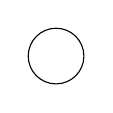
\begin{tikzpicture}[baseline=(current bounding box.center)]
        \begin{feynman}
            % draw an empty circle around the vertex a
            \node[circle,draw,inner sep=2.5mm] at (0,0) {};
        \end{feynman}
    \end{tikzpicture}
    - \frac{1}{8}\begin{tikzpicture}[baseline=(current bounding box.center)][baseline=(current bounding box.center)]
        \begin{feynman}
            \vertex (e) at (0,0);
            \diagram* {
                (e) -- [out=135,in=225,loop,min distance=1cm] e, % Left loop
                (e) -- [out=45,in=-45,loop,min distance=1cm] e, % Right loop
            };
        \end{feynman}
    \end{tikzpicture} - \frac{1}{48}
\begin{tikzpicture}[baseline=(current bounding box.center)][baseline=(current bounding box.center)]
        \begin{feynman}
            \vertex (a) at (0,0);
            % draw tree loops at vertex a, a three leaf clover 
            \diagram* {
                % Adjusted loop paths to manually create the desired "three leaf clover" shape
                (a) -- [out=135,in=225,loop,min distance=1cm] a, % Left loop
                (a) -- [out=45,in=-45,loop,min distance=1cm] a, % Right loop
                (a) -- [out=45,in=-235,loop,min distance=1cm] a, % Top loop
            };
        \end{feynman}
    \end{tikzpicture} + \frac{1}{8}\begin{tikzpicture}[baseline=(current bounding box.center)]
        \begin{feynman}
            \vertex (a) at (0,0);
            \vertex (b) at (0.5,0);
            \diagram* {
                % left loop at vertex a
                (a) -- [out=135,in=225,loop,min distance=1cm] a,
                (a) -- (b),
                % right loop at vertex b
                (b) -- [out=45,in=-45,loop,min distance=1cm] b,
            };
        \end{feynman}
    \end{tikzpicture} +  \frac{1}{12}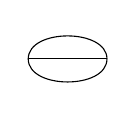
\begin{tikzpicture}[baseline=(current bounding box.center)]
        \begin{feynman}
            \vertex (a) at (0,0);
            \vertex (b) at (1,0);
            \diagram* {
                % draw four lines connecting a and b all curved
                (a) -- [out=90,in=90] (b),
                (a) -- [out=-90,in=-90] (b),
                (a) -- (b),
            };
        \end{feynman}
    \end{tikzpicture} \nonumber \\
    &+ \frac{1}{384}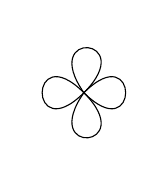
\begin{tikzpicture}[baseline=(current bounding box.center)]
        \begin{feynman}
            \vertex (a) at (0,0);
            % 4 leaf clover at vertex a
            \diagram* {
                % Adjusted loop paths to manually create the desired "four leaf clover" shape
                (a) -- [out=135,in=225,loop,min distance=1cm] a, % Left loop
                (a) -- [out=45,in=-45,loop,min distance=1cm] a, % Right loop
                (a) -- [out=45,in=-235,loop,min distance=1cm] a, % Top right loop
                (a) -- [out=235,in=-45,loop,min distance=1cm] a, % Top left loop
            };
        \end{feynman}
    \end{tikzpicture} \nonumber + \frac{1}{96}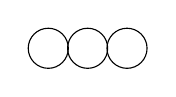
\begin{tikzpicture}[baseline=(current bounding box.center)]
        \begin{feynman}
            % circle connecting a and b
            \node[circle,draw,inner sep=1.8mm] at (0,0) {};
            \node[circle,draw,inner sep=1.8mm] at (0.5,0) {};
            \node[circle,draw,inner sep=1.8mm] at (1,0) {};
        \end{feynman}
    \end{tikzpicture} + \frac{1}{48}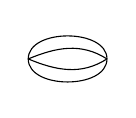
\begin{tikzpicture}[baseline=(current bounding box.center)]
        \begin{feynman}
            \vertex (a) at (0,0);
            \vertex (b) at (1,0);
            \diagram* {
                % draw four lines connecting a and b all curved
                (a) -- [out=22.5,in=147.5] (b),
                (a) -- [out=-22.5,in=-147.5] (b),
                (a) -- [out=90,in=90] (b),
                (a) -- [out=-90,in=-90] (b),
            };
        \end{feynman}
    \end{tikzpicture} + \frac{1}{32}\begin{tikzpicture}[baseline=(current bounding box.center)]
        \begin{feynman}
            \vertex (a) at (0,0);
            \vertex (b) at (0.5,0);
            \diagram* {
                % top left root 
                (a) -- [out=90,in=180,loop,min distance=1cm] a,
                % bottom left root
                (a) -- [out=-90,in=180,loop,min distance=1cm] a,
                (a) -- (b),
                % right loop at vertex b
                (b) -- [out=45,in=-45,loop,min distance=1cm] b,
            };
        \end{feynman}
    \end{tikzpicture} \nonumber \\ 
    &+ \frac{1}{12}\begin{tikzpicture}[baseline=(current bounding box.center)]
        \begin{feynman}
            \vertex (a) at (0,0);
            \vertex (b) at (1,0);
            \diagram* {
                % draw four lines connecting a and b all curved
                (a) -- [out=90,in=90] (b),
                (a) -- [out=-90,in=-90] (b),
                (a) -- (b),
                % left loop at vertex a
                (a) -- [out=135,in=225,loop,min distance=1.5cm] a,
            };
        \end{feynman}
    \end{tikzpicture} + \mathcal{O}(\bm{\Lambda^{(10)}}) \\
    &= -H_{0} + \log \sqrt{\abs{2\pi \bm{D}}} - \frac{1}{8}\bm{\Lambda^{(4)}}_{ijkl}\bm{D}_{ij}\bm{D}_{kl} - \frac{1}{48}\bm{\Lambda^{(6)}}_{ijklmn}\bm{D}_{ij}\bm{D}_{kl}\bm{D}_{mn} \\ 
    &+ \frac{1}{8}\bm{\Lambda^{(3)}}_{ijk}\bm{\Lambda^{(3)}}_{lmn}\bm{D}_{ij}\bm{D}_{kl}\bm{D}_{mn} - \frac{1}{384}\bm{\Lambda^{(8)}}_{ijklmnpq}\bm{D}_{ij}\bm{D}_{kl}\bm{D}_{mn}\bm{D}_{pq} \nonumber \\
    &+ \frac{1}{96}\bm{\Lambda^{(4)}}_{ijkl}\bm{\Lambda^{(4)}}_{mnop}\bm{D}_{ij}\bm{D}_{km}\bm{D}_{ln}\bm{D}_{op} + \frac{1}{48}\bm{\Lambda^{(4)}}_{ijkl}\bm{\Lambda^{(4)}}_{mnop}\bm{D}_{im}\bm{D}_{jn}\bm{D}_{ko}\bm{D}_{lp} \nonumber \\
    &+ \frac{1}{32}\bm{\Lambda^{(5)}}_{ijklm}\bm{\Lambda^{(3)}}_{nop}\bm{D}_{ij}\bm{D}_{kl}\bm{D}_{mn}\bm{D}_{op} + \frac{1}{12}\bm{\Lambda^{(5)}}_{ijklm}\bm{\Lambda^{(3)}}_{nop}\bm{D}_{ij}\bm{D}_{kn}\bm{D}_{lo}\bm{D}_{mp} + \mathcal{O}(\bm{\Lambda^{(10)}}) \nonumber
\end{align}
\textcolor{red}{Add the other 3rd order diagram}
    

We recall that, repeated indices are summed over under the Einstein summation convention. 
We can continue to go up till the correction term we want.

\vspace*{0.5cm}
To test this numerically we used Python. 
Using $N = 10, \bm{\theta}_{1} = 2, \theta_{2} = 5, \epsilon = \mathcal{N}(0, \sigma)$, and $\bm{X} = \mathcal{N}(0, 1)$, we generated the data set.

% MCMC results
% beta = 2.340
% log sigma = 3.121

% IFT results
% [2.34454322 3.02591931]
\vspace*{0.5cm}
We first ran a Markov Chain Monte Carlo (MCMC) simulation to estimate the regression coefficients.
The MCMC simulation yielded $\bm{\beta} = 2.340$ and $\log \sigma = 3.121$.
We then used the diagrammatic expansion technique to calculate the moments of the field.
The technique yielded $\bm{\beta} = 2.34454322$ and $\log \sigma = 3.02591931$.
The two results are in good agreement, with the IFT result being slightly higher than the MCMC result.

% ift result for Z
% ln(Z) = -19.958436807763317 (Z = 2.1486269907383194e-09)
% numerical result for Z
% ln Z:  -19.91886605407998 Z:  2.2353543980750245e-09

\vspace*{0.5cm}
Using the diagrammatic expansion technique, we calculated the partition function to be $\log Z = -19.958436807763317$.
We then compared this to the numerical result, which was $\log Z = -19.91886605407998$.
The two results are in good agreement, with the numerical result being slightly higher than the IFT result.

% \begin{center}
%     \begin{figure}[h]
%         \includegraphics[scale=0.3]{LinRegPlots.png}
%         \caption{Linear Regression Plots}
%     \end{figure}
% \end{center}

We compare the results of the MCMC simulation and the IFT technique in the plots above.
The numbered runs represent the 4 chains runned in the MCMC simulation and P1 represents the numerical result and P2 represents the IFT result.
We see that the two results are in good agreement, with the IFT results being able to capture the underlying trend in the data.

\section{Conclusion}

Information Field Theory is a powerful tool for inferring the moments of a random field, given a perturbatively non-Gaussian distribution. The diagrammatic expansion technique allows for the calculation of the moments of the field by summing over all possible diagrams that can be formed from the nth-order terms in the Hamiltonian.
The technique is particularly useful in cases where the partition function cannot be computed in a closed-form analytical expression, as it provides a method to extract information about the moments from the partition function up to a certain order of accuracy.
The technique can be applied to a wide range of problems, including linear regression, where it can be used to estimate the regression coefficients given the observed data and the design matrix.
The closed diagram expansion technique allows for the calculation of the moments of the field by summing over all possible closed diagrams that can be formed from the nth-order terms in the Hamiltonian.
The technique is particularly useful in cases where the partition function cannot be computed in a closed-form analytical expression, as it provides a method to extract information about the moments from the partition function up to a certain order of accuracy.


\subsection{Future Work}
We plan to explore the diagrammatic expansion technique in higher-dimensional cases, where the field is defined on a continuous underlying space.
We also plan to investigate the use of basis functions for more efficient calculations and not need to solve complicated integrals.
We wish to test the technique on other named distributions to see if it can be applied more broadly.

\subsubsection{Basis Functions}

The basis functions are a set of functions that span the space of the field.

We want to find functions $\phi_{i}(x)$ such that
\begin{equation}
    \int dx \, \phi_{i}(x)\phi_{j}(x) = \delta_{ij}
\end{equation}
so that 
\begin{equation}
    f(x) = \sum_{k} c_{k}\phi_{k}(x)
\end{equation}

We want to find such functins so that the following holds
\begin{equation}
    \int_{-\infty}^{\infty} dx \, f(x)P(x) = \sum_{k} c_{k}\int_{-\infty}^{\infty} dx \, \phi_{k}(x)P(x) = \sum_{k} c_{k}\int_{-\infty}^{\infty} dx \, \phi_{k}(x)\frac{e^{-H(x)}}{Z}
\end{equation}
If we can find exponential basis functions, then the basis functions could be absorbed into the $P(x)$ term.
This exponential basis functions would be of the form $e^{kax}$, where $a$ is some expression, and would act as the pertubation term in the Hamiltonian.
\begin{equation}
    \sum_{k} c_{k}\int_{-\infty}^{\infty} dx \, \frac{e^{kax}e^{-H(x)}}{Z} = \sum_{k} c_{k}\int_{-\infty}^{\infty} dx \, \frac{e^{-H(x) + kax}}{Z}
\end{equation}
Then the integral just becomes the sum of diagrams dependant on the basis functions times the coefficients of the basis functions.

\vspace*{0.5cm}
Some functions would have basis functions of the form $x^{kax}$, where $a$ is some expression, and so the integral then just becomes the sume of moments of the field times the coefficients of the basis functions.

\end{document}
